\documentclass[twoside]{book}

% Packages required by doxygen
\usepackage{calc}
\usepackage{doxygen}
\usepackage{graphicx}
\usepackage[utf8]{inputenc}
\usepackage{makeidx}
\usepackage{multicol}
\usepackage{multirow}
\usepackage{textcomp}
\usepackage[table]{xcolor}

% Font selection
\usepackage[T1]{fontenc}
\usepackage{mathptmx}
\usepackage[scaled=.90]{helvet}
\usepackage{courier}
\usepackage{amssymb}
\usepackage{sectsty}
\renewcommand{\familydefault}{\sfdefault}
\allsectionsfont{%
  \fontseries{bc}\selectfont%
  \color{darkgray}%
}
\renewcommand{\DoxyLabelFont}{%
  \fontseries{bc}\selectfont%
  \color{darkgray}%
}

% Page & text layout
\usepackage{geometry}
\geometry{%
  a4paper,%
  top=2.5cm,%
  bottom=2.5cm,%
  left=2.5cm,%
  right=2.5cm%
}
\tolerance=750
\hfuzz=15pt
\hbadness=750
\setlength{\emergencystretch}{15pt}
\setlength{\parindent}{0cm}
\setlength{\parskip}{0.2cm}
\makeatletter
\renewcommand{\paragraph}{%
  \@startsection{paragraph}{4}{0ex}{-1.0ex}{1.0ex}{%
    \normalfont\normalsize\bfseries\SS@parafont%
  }%
}
\renewcommand{\subparagraph}{%
  \@startsection{subparagraph}{5}{0ex}{-1.0ex}{1.0ex}{%
    \normalfont\normalsize\bfseries\SS@subparafont%
  }%
}
\makeatother

% Headers & footers
\usepackage{fancyhdr}
\pagestyle{fancyplain}
\fancyhead[LE]{\fancyplain{}{\bfseries\thepage}}
\fancyhead[CE]{\fancyplain{}{}}
\fancyhead[RE]{\fancyplain{}{\bfseries\leftmark}}
\fancyhead[LO]{\fancyplain{}{\bfseries\rightmark}}
\fancyhead[CO]{\fancyplain{}{}}
\fancyhead[RO]{\fancyplain{}{\bfseries\thepage}}
\fancyfoot[LE]{\fancyplain{}{}}
\fancyfoot[CE]{\fancyplain{}{}}
\fancyfoot[RE]{\fancyplain{}{\bfseries\scriptsize Generated on Wed May 18 2016 21\-:27\-:12 for Chef interpreter by Doxygen }}
\fancyfoot[LO]{\fancyplain{}{\bfseries\scriptsize Generated on Wed May 18 2016 21\-:27\-:12 for Chef interpreter by Doxygen }}
\fancyfoot[CO]{\fancyplain{}{}}
\fancyfoot[RO]{\fancyplain{}{}}
\renewcommand{\footrulewidth}{0.4pt}
\renewcommand{\chaptermark}[1]{%
  \markboth{#1}{}%
}
\renewcommand{\sectionmark}[1]{%
  \markright{\thesection\ #1}%
}

% Indices & bibliography
\usepackage{natbib}
\usepackage[titles]{tocloft}
\setcounter{tocdepth}{3}
\setcounter{secnumdepth}{5}
\makeindex

% Hyperlinks (required, but should be loaded last)
\usepackage{ifpdf}
\ifpdf
  \usepackage[pdftex,pagebackref=true]{hyperref}
\else
  \usepackage[ps2pdf,pagebackref=true]{hyperref}
\fi
\hypersetup{%
  colorlinks=true,%
  linkcolor=blue,%
  citecolor=blue,%
  unicode%
}

% Custom commands
\newcommand{\clearemptydoublepage}{%
  \newpage{\pagestyle{empty}\cleardoublepage}%
}


%===== C O N T E N T S =====

\begin{document}

% Titlepage & ToC
\hypersetup{pageanchor=false}
\pagenumbering{roman}
\begin{titlepage}
\vspace*{7cm}
\begin{center}%
{\Large Chef interpreter }\\
\vspace*{1cm}
{\large Generated by Doxygen 1.8.6}\\
\vspace*{0.5cm}
{\small Wed May 18 2016 21:27:12}\\
\end{center}
\end{titlepage}
\clearemptydoublepage
\tableofcontents
\clearemptydoublepage
\pagenumbering{arabic}
\hypersetup{pageanchor=true}

%--- Begin generated contents ---
\chapter{Chef interpreter}
\label{index}\hypertarget{index}{}\subsection*{Chef language}

Chef is stack-\/based esoteric programming language designed by David Morgan-\/\-Mar in 2002. Programs in Chef look like recipes, where variables are represented by ingredients and program's stacks are referred to as mixing bowls and baking dishes.

Full specification of the language can be found on \href{http://www.dangermouse.net/esoteric/chef.html}{\tt David Morgan-\/\-Mar's webpage} or on \href{http://search.cpan.org/~smueller/Acme-Chef/lib/Acme/Chef.pm}{\tt Steffan Mueller's interpreter pages}. \subsection*{Usage of the interpreter}

\subsubsection*{Command line arguments}

-\/i $<$file$>$ input file

-\/o $<$file$>$ output file

-\/v show also information about recipe

-\/t trace mode \subsubsection*{Example}

chef -\/i my\-Input.\-chef -\/o output.\-txt -\/v

\subsection*{Download}

\href{http://eckhaus.github.io/chef/}{\tt http\-://eckhaus.\-github.\-io/chef/}

\subsection*{Known issues}

Serves command is mandatory after every recipe.

{\itshape Róbert Eckhaus, M\-F\-F U\-K, 2016} 
\chapter{Module Index}
\section{Modules}
Here is a list of all modules\-:\begin{DoxyCompactList}
\item \contentsline{section}{Command}{\pageref{group__Command}}{}
\end{DoxyCompactList}

\chapter{Hierarchical Index}
\section{Class Hierarchy}
This inheritance list is sorted roughly, but not completely, alphabetically\-:\begin{DoxyCompactList}
\item \contentsline{section}{Command}{\pageref{structCommand}}{}
\item \contentsline{section}{Ingredient}{\pageref{classIngredient}}{}
\item \contentsline{section}{Jump}{\pageref{structJump}}{}
\item \contentsline{section}{Program}{\pageref{classProgram}}{}
\item \contentsline{section}{Recipe}{\pageref{classRecipe}}{}
\item stack\begin{DoxyCompactList}
\item \contentsline{section}{Dish}{\pageref{classDish}}{}
\begin{DoxyCompactList}
\item \contentsline{section}{Baking\-Dish}{\pageref{classBakingDish}}{}
\item \contentsline{section}{Mixing\-Bowl}{\pageref{classMixingBowl}}{}
\end{DoxyCompactList}
\end{DoxyCompactList}
\item \contentsline{section}{Stack\-Info}{\pageref{structStackInfo}}{}
\end{DoxyCompactList}

\chapter{Class Index}
\section{Class List}
Here are the classes, structs, unions and interfaces with brief descriptions\-:\begin{DoxyCompactList}
\item\contentsline{section}{\hyperlink{structCommand}{Command} \\*Stores command's name and arguments }{\pageref{structCommand}}{}
\item\contentsline{section}{\hyperlink{classDish}{Dish} \\*Stack of Ingredients }{\pageref{classDish}}{}
\item\contentsline{section}{\hyperlink{classIngredient}{Ingredient} \\*Structure for program's variables -\/ ingredients }{\pageref{classIngredient}}{}
\item\contentsline{section}{\hyperlink{structJump}{Jump} \\*Describes a single jump (used in loop statements) }{\pageref{structJump}}{}
\item\contentsline{section}{\hyperlink{classProgram}{Program} \\*Parses and interprets the source code. Handles the execution of the main script }{\pageref{classProgram}}{}
\item\contentsline{section}{\hyperlink{classRecipe}{Recipe} \\*Stores all the information about recipes \& executes their commands }{\pageref{classRecipe}}{}
\item\contentsline{section}{\hyperlink{structStackInfo}{Stack\-Info} \\*Item stored in stack (\hyperlink{classDish}{Dish}), stores value and type of \hyperlink{classIngredient}{Ingredient} }{\pageref{structStackInfo}}{}
\end{DoxyCompactList}

\chapter{Module Documentation}
\hypertarget{group__Command}{\section{Command}
\label{group__Command}\index{Command@{Command}}
}


Chef language command as described \href{http://www.dangermouse.net/esoteric/chef.html}{\tt here}.  


\subsection*{Functions}
\begin{DoxyCompactItemize}
\item 
void \hyperlink{group__Command_ga003607cfe3ab13de0bc6b85d659856bc}{Recipe\-::do\-Jump} (\hyperlink{structJump}{Jump} \&j)
\item 
void \hyperlink{group__Command_gadad4684f1b60dbabd7ac9b8ac9816d32}{Recipe\-::do\-Until} (\hyperlink{structJump}{Jump} \&j)
\item 
void \hyperlink{group__Command_ga5119039470b26422e6ec843515d4a720}{Recipe\-::take\-From\-Fridge} (const string \&ingredient)
\item 
void \hyperlink{group__Command_ga928df02758f8f959f4beeb153ddde7d6}{Recipe\-::put} (const string \&ingredient, int bowl\-No=1)
\item 
void \hyperlink{group__Command_gaf5f825d69a4a19837a0714715710734a}{Recipe\-::fold} (const string \&ingredient, int bowl\-No=1)
\item 
void \hyperlink{group__Command_ga385cb79270fb9c857256ef79ff65010e}{Recipe\-::add} (const string \&ingredient, int bowl\-No=1)
\item 
void \hyperlink{group__Command_ga31fa0f785049498f85ab6e299217c7ab}{Recipe\-::remove} (const string \&ingredient, int bowl\-No=1)
\item 
void \hyperlink{group__Command_ga276a0e85ac154372bf1c4cdaf7304d09}{Recipe\-::combine} (const string \&ingredient, int bowl\-No=1)
\item 
void \hyperlink{group__Command_ga5d32e4fe23897d4dbb0b10eb4821baeb}{Recipe\-::divide} (const string \&ingredient, int bowl\-No=1)
\item 
void \hyperlink{group__Command_ga7c657ea9ec19dfb55292a7474fe12511}{Recipe\-::add\-Dry} (int bowl\-No=1)
\item 
void \hyperlink{group__Command_gaf44790b96aebd727ff3d7ccbbf9ff568}{Recipe\-::liquify} (const string \&ingredient)
\item 
void \hyperlink{group__Command_ga5b48c67eb04fc71c199bdf611c387c9e}{Recipe\-::stir} (int times, int bowl\-No=1)
\item 
void \hyperlink{group__Command_ga2678e5c7db062e186ca947018050f5c2}{Recipe\-::stir\-Ingredient} (const string \&ingredient, int bowl\-No=1)
\item 
void \hyperlink{group__Command_gad9a02b3a48b606ba17dc91337c3f64c2}{Recipe\-::mix} (int bowl\-No=1)
\item 
void \hyperlink{group__Command_gae041e0eb15d1e40fe513b53803810dac}{Recipe\-::clean} (int bowl\-No=1)
\item 
void \hyperlink{group__Command_ga03848074a9e527439e6381e47d9f3749}{Recipe\-::pour} (int bowl\-No=1, int dish\-No=1)
\item 
int \hyperlink{group__Command_ga2485acb9291f44d16222f15a75ff27fb}{Recipe\-::call} (const string \&aux)
\item 
void \hyperlink{group__Command_ga4889710ccae668fb039e4dfa0ea2dae7}{Recipe\-::set\-Aside} ()
\end{DoxyCompactItemize}


\subsection{Detailed Description}
Chef language command as described \href{http://www.dangermouse.net/esoteric/chef.html}{\tt here}. 

\subsection{Function Documentation}
\hypertarget{group__Command_ga385cb79270fb9c857256ef79ff65010e}{\index{Command@{Command}!add@{add}}
\index{add@{add}!Command@{Command}}
\subsubsection[{add}]{\setlength{\rightskip}{0pt plus 5cm}void Recipe\-::add (
\begin{DoxyParamCaption}
\item[{const string \&}]{ingredient, }
\item[{int}]{bowl\-No = {\ttfamily 1}}
\end{DoxyParamCaption}
)\hspace{0.3cm}{\ttfamily [private]}}}\label{group__Command_ga385cb79270fb9c857256ef79ff65010e}
Add value of given ingredient to the value on the top of the mixing bowl \hypertarget{group__Command_ga7c657ea9ec19dfb55292a7474fe12511}{\index{Command@{Command}!add\-Dry@{add\-Dry}}
\index{add\-Dry@{add\-Dry}!Command@{Command}}
\subsubsection[{add\-Dry}]{\setlength{\rightskip}{0pt plus 5cm}void Recipe\-::add\-Dry (
\begin{DoxyParamCaption}
\item[{int}]{bowl\-No = {\ttfamily 1}}
\end{DoxyParamCaption}
)\hspace{0.3cm}{\ttfamily [private]}}}\label{group__Command_ga7c657ea9ec19dfb55292a7474fe12511}
Place the sum of quantities of dry ingredients on top of the mixing bowl \hypertarget{group__Command_ga2485acb9291f44d16222f15a75ff27fb}{\index{Command@{Command}!call@{call}}
\index{call@{call}!Command@{Command}}
\subsubsection[{call}]{\setlength{\rightskip}{0pt plus 5cm}int Recipe\-::call (
\begin{DoxyParamCaption}
\item[{const string \&}]{aux}
\end{DoxyParamCaption}
)\hspace{0.3cm}{\ttfamily [private]}}}\label{group__Command_ga2485acb9291f44d16222f15a75ff27fb}
Call auxliary recipe \hypertarget{group__Command_gae041e0eb15d1e40fe513b53803810dac}{\index{Command@{Command}!clean@{clean}}
\index{clean@{clean}!Command@{Command}}
\subsubsection[{clean}]{\setlength{\rightskip}{0pt plus 5cm}void Recipe\-::clean (
\begin{DoxyParamCaption}
\item[{int}]{bowl\-No = {\ttfamily 1}}
\end{DoxyParamCaption}
)\hspace{0.3cm}{\ttfamily [private]}}}\label{group__Command_gae041e0eb15d1e40fe513b53803810dac}
Empty the stack \hypertarget{group__Command_ga276a0e85ac154372bf1c4cdaf7304d09}{\index{Command@{Command}!combine@{combine}}
\index{combine@{combine}!Command@{Command}}
\subsubsection[{combine}]{\setlength{\rightskip}{0pt plus 5cm}void Recipe\-::combine (
\begin{DoxyParamCaption}
\item[{const string \&}]{ingredient, }
\item[{int}]{bowl\-No = {\ttfamily 1}}
\end{DoxyParamCaption}
)\hspace{0.3cm}{\ttfamily [private]}}}\label{group__Command_ga276a0e85ac154372bf1c4cdaf7304d09}
Multiply the value on the top of the mixing bowl by given ingredient's value \hypertarget{group__Command_ga5d32e4fe23897d4dbb0b10eb4821baeb}{\index{Command@{Command}!divide@{divide}}
\index{divide@{divide}!Command@{Command}}
\subsubsection[{divide}]{\setlength{\rightskip}{0pt plus 5cm}void Recipe\-::divide (
\begin{DoxyParamCaption}
\item[{const string \&}]{ingredient, }
\item[{int}]{bowl\-No = {\ttfamily 1}}
\end{DoxyParamCaption}
)\hspace{0.3cm}{\ttfamily [private]}}}\label{group__Command_ga5d32e4fe23897d4dbb0b10eb4821baeb}
Divide the value on the top of the mixing bowl by given ingredient's value \hypertarget{group__Command_ga003607cfe3ab13de0bc6b85d659856bc}{\index{Command@{Command}!do\-Jump@{do\-Jump}}
\index{do\-Jump@{do\-Jump}!Command@{Command}}
\subsubsection[{do\-Jump}]{\setlength{\rightskip}{0pt plus 5cm}void Recipe\-::do\-Jump (
\begin{DoxyParamCaption}
\item[{{\bf Jump} \&}]{j}
\end{DoxyParamCaption}
)\hspace{0.3cm}{\ttfamily [private]}}}\label{group__Command_ga003607cfe3ab13de0bc6b85d659856bc}
Do jump (check condition) \hypertarget{group__Command_gadad4684f1b60dbabd7ac9b8ac9816d32}{\index{Command@{Command}!do\-Until@{do\-Until}}
\index{do\-Until@{do\-Until}!Command@{Command}}
\subsubsection[{do\-Until}]{\setlength{\rightskip}{0pt plus 5cm}void Recipe\-::do\-Until (
\begin{DoxyParamCaption}
\item[{{\bf Jump} \&}]{j}
\end{DoxyParamCaption}
)\hspace{0.3cm}{\ttfamily [private]}}}\label{group__Command_gadad4684f1b60dbabd7ac9b8ac9816d32}
End of jump (jump back to loop begining label) \hypertarget{group__Command_gaf5f825d69a4a19837a0714715710734a}{\index{Command@{Command}!fold@{fold}}
\index{fold@{fold}!Command@{Command}}
\subsubsection[{fold}]{\setlength{\rightskip}{0pt plus 5cm}void Recipe\-::fold (
\begin{DoxyParamCaption}
\item[{const string \&}]{ingredient, }
\item[{int}]{bowl\-No = {\ttfamily 1}}
\end{DoxyParamCaption}
)\hspace{0.3cm}{\ttfamily [private]}}}\label{group__Command_gaf5f825d69a4a19837a0714715710734a}
Remove the top value of the mixing bowl and store it in ingredient \hypertarget{group__Command_gaf44790b96aebd727ff3d7ccbbf9ff568}{\index{Command@{Command}!liquify@{liquify}}
\index{liquify@{liquify}!Command@{Command}}
\subsubsection[{liquify}]{\setlength{\rightskip}{0pt plus 5cm}void Recipe\-::liquify (
\begin{DoxyParamCaption}
\item[{const string \&}]{ingredient}
\end{DoxyParamCaption}
)\hspace{0.3cm}{\ttfamily [private]}}}\label{group__Command_gaf44790b96aebd727ff3d7ccbbf9ff568}
Set ingredient's type to liquid (A\-S\-C\-I\-I character) \hypertarget{group__Command_gad9a02b3a48b606ba17dc91337c3f64c2}{\index{Command@{Command}!mix@{mix}}
\index{mix@{mix}!Command@{Command}}
\subsubsection[{mix}]{\setlength{\rightskip}{0pt plus 5cm}void Recipe\-::mix (
\begin{DoxyParamCaption}
\item[{int}]{bowl\-No = {\ttfamily 1}}
\end{DoxyParamCaption}
)\hspace{0.3cm}{\ttfamily [private]}}}\label{group__Command_gad9a02b3a48b606ba17dc91337c3f64c2}
Shuffle the stack randomly \hypertarget{group__Command_ga03848074a9e527439e6381e47d9f3749}{\index{Command@{Command}!pour@{pour}}
\index{pour@{pour}!Command@{Command}}
\subsubsection[{pour}]{\setlength{\rightskip}{0pt plus 5cm}void Recipe\-::pour (
\begin{DoxyParamCaption}
\item[{int}]{bowl\-No = {\ttfamily 1}, }
\item[{int}]{dish\-No = {\ttfamily 1}}
\end{DoxyParamCaption}
)\hspace{0.3cm}{\ttfamily [private]}}}\label{group__Command_ga03848074a9e527439e6381e47d9f3749}
Copy the stack into the baking dish (output stack) \hypertarget{group__Command_ga928df02758f8f959f4beeb153ddde7d6}{\index{Command@{Command}!put@{put}}
\index{put@{put}!Command@{Command}}
\subsubsection[{put}]{\setlength{\rightskip}{0pt plus 5cm}void Recipe\-::put (
\begin{DoxyParamCaption}
\item[{const string \&}]{ingredient, }
\item[{int}]{bowl\-No = {\ttfamily 1}}
\end{DoxyParamCaption}
)\hspace{0.3cm}{\ttfamily [private]}}}\label{group__Command_ga928df02758f8f959f4beeb153ddde7d6}
Put ingredient into the mixing bowl \hypertarget{group__Command_ga31fa0f785049498f85ab6e299217c7ab}{\index{Command@{Command}!remove@{remove}}
\index{remove@{remove}!Command@{Command}}
\subsubsection[{remove}]{\setlength{\rightskip}{0pt plus 5cm}void Recipe\-::remove (
\begin{DoxyParamCaption}
\item[{const string \&}]{ingredient, }
\item[{int}]{bowl\-No = {\ttfamily 1}}
\end{DoxyParamCaption}
)\hspace{0.3cm}{\ttfamily [private]}}}\label{group__Command_ga31fa0f785049498f85ab6e299217c7ab}
Subtract value of given ingredient from the value on the top of the mixing bowl \hypertarget{group__Command_ga4889710ccae668fb039e4dfa0ea2dae7}{\index{Command@{Command}!set\-Aside@{set\-Aside}}
\index{set\-Aside@{set\-Aside}!Command@{Command}}
\subsubsection[{set\-Aside}]{\setlength{\rightskip}{0pt plus 5cm}void Recipe\-::set\-Aside (
\begin{DoxyParamCaption}
{}
\end{DoxyParamCaption}
)\hspace{0.3cm}{\ttfamily [private]}}}\label{group__Command_ga4889710ccae668fb039e4dfa0ea2dae7}
Break the innermost loop \hypertarget{group__Command_ga5b48c67eb04fc71c199bdf611c387c9e}{\index{Command@{Command}!stir@{stir}}
\index{stir@{stir}!Command@{Command}}
\subsubsection[{stir}]{\setlength{\rightskip}{0pt plus 5cm}void Recipe\-::stir (
\begin{DoxyParamCaption}
\item[{int}]{times, }
\item[{int}]{bowl\-No = {\ttfamily 1}}
\end{DoxyParamCaption}
)\hspace{0.3cm}{\ttfamily [private]}}}\label{group__Command_ga5b48c67eb04fc71c199bdf611c387c9e}
Move the top of the stack n positions deeper into the stack \hypertarget{group__Command_ga2678e5c7db062e186ca947018050f5c2}{\index{Command@{Command}!stir\-Ingredient@{stir\-Ingredient}}
\index{stir\-Ingredient@{stir\-Ingredient}!Command@{Command}}
\subsubsection[{stir\-Ingredient}]{\setlength{\rightskip}{0pt plus 5cm}void Recipe\-::stir\-Ingredient (
\begin{DoxyParamCaption}
\item[{const string \&}]{ingredient, }
\item[{int}]{bowl\-No = {\ttfamily 1}}
\end{DoxyParamCaption}
)\hspace{0.3cm}{\ttfamily [private]}}}\label{group__Command_ga2678e5c7db062e186ca947018050f5c2}
Stir the value of ingredient into the stack \hypertarget{group__Command_ga5119039470b26422e6ec843515d4a720}{\index{Command@{Command}!take\-From\-Fridge@{take\-From\-Fridge}}
\index{take\-From\-Fridge@{take\-From\-Fridge}!Command@{Command}}
\subsubsection[{take\-From\-Fridge}]{\setlength{\rightskip}{0pt plus 5cm}void Recipe\-::take\-From\-Fridge (
\begin{DoxyParamCaption}
\item[{const string \&}]{ingredient}
\end{DoxyParamCaption}
)\hspace{0.3cm}{\ttfamily [private]}}}\label{group__Command_ga5119039470b26422e6ec843515d4a720}
Read value from standard input, store it in ingredient 
\chapter{Class Documentation}
\hypertarget{structCommand}{\section{Command Struct Reference}
\label{structCommand}\index{Command@{Command}}
}


Stores command's name and arguments.  




{\ttfamily \#include $<$Recipe.\-h$>$}

\subsection*{Public Member Functions}
\begin{DoxyCompactItemize}
\item 
\hypertarget{structCommand_ad5baf9209de07797e8f6525a8d8b5eee}{{\bfseries Command} (string cmd, string arg1, string arg2)}\label{structCommand_ad5baf9209de07797e8f6525a8d8b5eee}

\end{DoxyCompactItemize}
\subsection*{Public Attributes}
\begin{DoxyCompactItemize}
\item 
\hypertarget{structCommand_aff4def5cb9cabcb8b719ccb472c527f5}{string {\bfseries cmd}}\label{structCommand_aff4def5cb9cabcb8b719ccb472c527f5}

\item 
\hypertarget{structCommand_af859040272fe89b1640db987bf06d535}{string {\bfseries arg1}}\label{structCommand_af859040272fe89b1640db987bf06d535}

\item 
\hypertarget{structCommand_a415cd7a04e524df881e49d35cf0d5d09}{string {\bfseries arg2}}\label{structCommand_a415cd7a04e524df881e49d35cf0d5d09}

\end{DoxyCompactItemize}


\subsection{Detailed Description}
Stores command's name and arguments. 

The documentation for this struct was generated from the following file\-:\begin{DoxyCompactItemize}
\item 
/home/eckhaus/\-Desktop/cpp/zapoctak\-\_\-prod/source/include/Recipe.\-h\end{DoxyCompactItemize}

\hypertarget{classDish}{\section{Dish Class Reference}
\label{classDish}\index{Dish@{Dish}}
}


Stack of Ingredients.  




{\ttfamily \#include $<$Dish.\-h$>$}

Inheritance diagram for Dish\-:\begin{figure}[H]
\begin{center}
\leavevmode
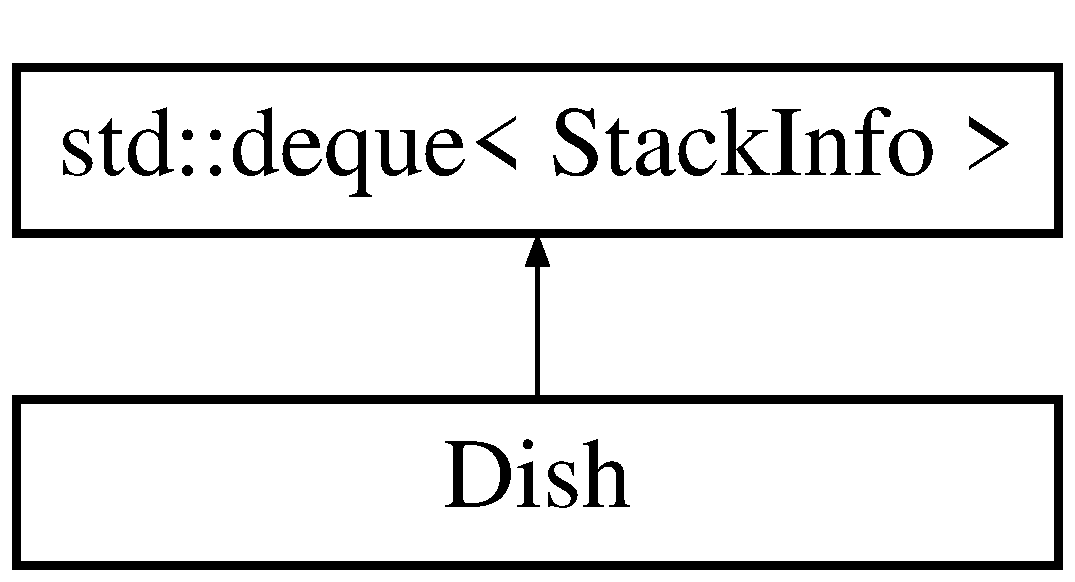
\includegraphics[height=2.000000cm]{classDish}
\end{center}
\end{figure}
\subsection*{Public Member Functions}
\begin{DoxyCompactItemize}
\item 
void \hyperlink{classDish_a1f67fe39855ea4899a110591f960745b}{print} (std\-::ostream $\ast$os)
\item 
bool \hyperlink{classDish_a437c63798f934fdc3c80037d77a0d51e}{pop\-Top} (\hyperlink{structStackInfo}{Stack\-Info} \&i)
\item 
void \hyperlink{classDish_ac0abbc375bf201a4267b3b57c82d2a8f}{append} (const \hyperlink{classDish}{Dish} \&d)
\item 
void \hyperlink{classDish_a41b6fc6a531325d36d4607546291386b}{liquify} ()
\item 
\hypertarget{classDish_afbec6d938ea55ca2a848bedd954faa59}{void {\bfseries stir} (unsigned int places)}\label{classDish_afbec6d938ea55ca2a848bedd954faa59}

\item 
void \hyperlink{classDish_a1c60aa114f084117df18578e58f0725d}{randomize} ()
\end{DoxyCompactItemize}
\subsection*{Public Attributes}
\begin{DoxyCompactItemize}
\item 
\hypertarget{classDish_a14264990a9a7bc34f61336eeb6dcfcbd}{int {\bfseries I\-D}}\label{classDish_a14264990a9a7bc34f61336eeb6dcfcbd}

\end{DoxyCompactItemize}


\subsection{Detailed Description}
Stack of Ingredients. 

\subsection{Member Function Documentation}
\hypertarget{classDish_ac0abbc375bf201a4267b3b57c82d2a8f}{\index{Dish@{Dish}!append@{append}}
\index{append@{append}!Dish@{Dish}}
\subsubsection[{append}]{\setlength{\rightskip}{0pt plus 5cm}void Dish\-::append (
\begin{DoxyParamCaption}
\item[{const {\bf Dish} \&}]{d}
\end{DoxyParamCaption}
)}}\label{classDish_ac0abbc375bf201a4267b3b57c82d2a8f}
Append stack d to the end of this stack \hypertarget{classDish_a41b6fc6a531325d36d4607546291386b}{\index{Dish@{Dish}!liquify@{liquify}}
\index{liquify@{liquify}!Dish@{Dish}}
\subsubsection[{liquify}]{\setlength{\rightskip}{0pt plus 5cm}void Dish\-::liquify (
\begin{DoxyParamCaption}
{}
\end{DoxyParamCaption}
)}}\label{classDish_a41b6fc6a531325d36d4607546291386b}
Convert all items in the stack to liquids (characters) \hypertarget{classDish_a437c63798f934fdc3c80037d77a0d51e}{\index{Dish@{Dish}!pop\-Top@{pop\-Top}}
\index{pop\-Top@{pop\-Top}!Dish@{Dish}}
\subsubsection[{pop\-Top}]{\setlength{\rightskip}{0pt plus 5cm}bool Dish\-::pop\-Top (
\begin{DoxyParamCaption}
\item[{{\bf Stack\-Info} \&}]{i}
\end{DoxyParamCaption}
)}}\label{classDish_a437c63798f934fdc3c80037d77a0d51e}
Pop top of the stack into i \hypertarget{classDish_a1f67fe39855ea4899a110591f960745b}{\index{Dish@{Dish}!print@{print}}
\index{print@{print}!Dish@{Dish}}
\subsubsection[{print}]{\setlength{\rightskip}{0pt plus 5cm}void Dish\-::print (
\begin{DoxyParamCaption}
\item[{std\-::ostream $\ast$}]{os}
\end{DoxyParamCaption}
)}}\label{classDish_a1f67fe39855ea4899a110591f960745b}
Print out the stack \hypertarget{classDish_a1c60aa114f084117df18578e58f0725d}{\index{Dish@{Dish}!randomize@{randomize}}
\index{randomize@{randomize}!Dish@{Dish}}
\subsubsection[{randomize}]{\setlength{\rightskip}{0pt plus 5cm}void Dish\-::randomize (
\begin{DoxyParamCaption}
{}
\end{DoxyParamCaption}
)}}\label{classDish_a1c60aa114f084117df18578e58f0725d}
Pushes top of the stack 'places' items deeper into the stack 

The documentation for this class was generated from the following files\-:\begin{DoxyCompactItemize}
\item 
/home/eckhaus/git/eckhaus.\-github.\-io/chef/source/include/Dish.\-h\item 
/home/eckhaus/git/eckhaus.\-github.\-io/chef/source/src/Dish.\-cpp\end{DoxyCompactItemize}

\hypertarget{classIngredient}{\section{Ingredient Class Reference}
\label{classIngredient}\index{Ingredient@{Ingredient}}
}


Structure for program's variables -\/ ingredients.  




{\ttfamily \#include $<$Ingredient.\-h$>$}

\subsection*{Public Member Functions}
\begin{DoxyCompactItemize}
\item 
\hyperlink{classIngredient_a738111e26d0765aabc92ebc036fad1d3}{Ingredient} ()
\item 
\hypertarget{classIngredient_af3acf81df28510c184f1f974f96c1471}{{\bfseries Ingredient} (string \hyperlink{classIngredient_a3fc00c5a7606e8e834d744676e38cdea}{name}, int \hyperlink{classIngredient_aa95e40564ad71f9ec536fb8d3fa3b839}{value}, Ingredient\-Type type)}\label{classIngredient_af3acf81df28510c184f1f974f96c1471}

\end{DoxyCompactItemize}
\subsection*{Public Attributes}
\begin{DoxyCompactItemize}
\item 
string \hyperlink{classIngredient_a3fc00c5a7606e8e834d744676e38cdea}{name}
\item 
int \hyperlink{classIngredient_aa95e40564ad71f9ec536fb8d3fa3b839}{value}
\item 
\hypertarget{classIngredient_a29a400e987a68bd02363b30b52e89710}{Ingredient\-Type {\bfseries type}}\label{classIngredient_a29a400e987a68bd02363b30b52e89710}

\end{DoxyCompactItemize}


\subsection{Detailed Description}
Structure for program's variables -\/ ingredients. 

\subsection{Constructor \& Destructor Documentation}
\hypertarget{classIngredient_a738111e26d0765aabc92ebc036fad1d3}{\index{Ingredient@{Ingredient}!Ingredient@{Ingredient}}
\index{Ingredient@{Ingredient}!Ingredient@{Ingredient}}
\subsubsection[{Ingredient}]{\setlength{\rightskip}{0pt plus 5cm}Ingredient\-::\-Ingredient (
\begin{DoxyParamCaption}
{}
\end{DoxyParamCaption}
)\hspace{0.3cm}{\ttfamily [inline]}}}\label{classIngredient_a738111e26d0765aabc92ebc036fad1d3}
Type, can be Liquid, Dry or Unspecified 

\subsection{Member Data Documentation}
\hypertarget{classIngredient_a3fc00c5a7606e8e834d744676e38cdea}{\index{Ingredient@{Ingredient}!name@{name}}
\index{name@{name}!Ingredient@{Ingredient}}
\subsubsection[{name}]{\setlength{\rightskip}{0pt plus 5cm}string Ingredient\-::name}}\label{classIngredient_a3fc00c5a7606e8e834d744676e38cdea}
Name of the ingredient \hypertarget{classIngredient_aa95e40564ad71f9ec536fb8d3fa3b839}{\index{Ingredient@{Ingredient}!value@{value}}
\index{value@{value}!Ingredient@{Ingredient}}
\subsubsection[{value}]{\setlength{\rightskip}{0pt plus 5cm}int Ingredient\-::value}}\label{classIngredient_aa95e40564ad71f9ec536fb8d3fa3b839}
Value of the ingredient 

The documentation for this class was generated from the following file\-:\begin{DoxyCompactItemize}
\item 
/home/eckhaus/\-Desktop/cpp/zapoctak\-\_\-prod/source/include/Ingredient.\-h\end{DoxyCompactItemize}

\hypertarget{structJump}{\section{Jump Struct Reference}
\label{structJump}\index{Jump@{Jump}}
}


Describes a single jump (used in loop statements)  




{\ttfamily \#include $<$Recipe.\-h$>$}

\subsection*{Public Attributes}
\begin{DoxyCompactItemize}
\item 
\hypertarget{structJump_aacc2efa25696a52f6f61f62267ab2f47}{int {\bfseries begin}}\label{structJump_aacc2efa25696a52f6f61f62267ab2f47}

\item 
\hypertarget{structJump_aa71cf756358c686638ffc89fa770d479}{int {\bfseries end}}\label{structJump_aa71cf756358c686638ffc89fa770d479}

\item 
\hypertarget{structJump_a17951d7947d33ea44e3bc961098721b6}{string {\bfseries verb}}\label{structJump_a17951d7947d33ea44e3bc961098721b6}

\item 
\hypertarget{structJump_a3a86e53486aa1fd1e53ce1e4419b72b0}{string {\bfseries begin\-\_\-ingredient}}\label{structJump_a3a86e53486aa1fd1e53ce1e4419b72b0}

\item 
\hypertarget{structJump_afbc8174b322f14a877dd6f276d078bb1}{string {\bfseries end\-\_\-ingredient}}\label{structJump_afbc8174b322f14a877dd6f276d078bb1}

\end{DoxyCompactItemize}


\subsection{Detailed Description}
Describes a single jump (used in loop statements) 

The documentation for this struct was generated from the following file\-:\begin{DoxyCompactItemize}
\item 
/home/eckhaus/git/eckhaus.\-github.\-io/chef/source/include/Recipe.\-h\end{DoxyCompactItemize}

\hypertarget{classProgram}{\section{Program Class Reference}
\label{classProgram}\index{Program@{Program}}
}


Parses and interprets the source code. Handles the execution of the main script.  




{\ttfamily \#include $<$Program.\-h$>$}

\subsection*{Public Member Functions}
\begin{DoxyCompactItemize}
\item 
void \hyperlink{classProgram_a7e845a6184bade97aead63d2e14c5040}{parse} ()
\item 
\hypertarget{classProgram_aee67cabb04f36e7e0f059c1976d55601}{{\bfseries Program} (string input, string output, bool v, bool t)}\label{classProgram_aee67cabb04f36e7e0f059c1976d55601}

\end{DoxyCompactItemize}
\subsection*{Private Member Functions}
\begin{DoxyCompactItemize}
\item 
void \hyperlink{classProgram_ad5a95ba2b5f9caa0555d7d24c475f502}{normalize} (string \&s)
\item 
Ingredient\-Type \hyperlink{classProgram_aa97b3ca0f048f04847e6be90581cf756}{type\-From\-String} (const string \&s)
\item 
void \hyperlink{classProgram_a20fc155df19b3cfc73901e31f2fad53d}{set\-Up\-Regex} ()
\item 
bool \hyperlink{classProgram_a4e8ea37034e515f7c21d3fb3cc119765}{Load\-Header} (\hyperlink{classRecipe}{Recipe} \&r)
\item 
void \hyperlink{classProgram_a277650f0e2ae017e8171aee4fbde0ae2}{Load\-Ingredients} (\hyperlink{classRecipe}{Recipe} \&r)
\item 
bool \hyperlink{classProgram_a28d7594324677db5e10aff47fa97f593}{Load\-Recipe} (\hyperlink{classRecipe}{Recipe} \&r)
\item 
\hypertarget{classProgram_a7ee14d6b0460dcb1501884db70972657}{bool {\bfseries parse\-Command} (\hyperlink{classRecipe}{Recipe} \&r, string \&line)}\label{classProgram_a7ee14d6b0460dcb1501884db70972657}

\end{DoxyCompactItemize}
\subsection*{Private Attributes}
\begin{DoxyCompactItemize}
\item 
\hyperlink{classRecipe}{Recipe} \hyperlink{classProgram_a414bb40153c7da0e1815b7140c4aa454}{main\-\_\-recipe}
\item 
bool \hyperlink{classProgram_a3787a8712d4c75b6b5f0e81a5e4f6fdc}{print\-Parser\-Output} = false
\item 
bool \hyperlink{classProgram_a4addd74ec821dc25e804fa2096b7fa59}{print\-Program\-Info} = false
\item 
bool \hyperlink{classProgram_ad4371cad6bc5c0f4cd232007a2324205}{print\-Auxiliary\-Programs} = true
\item 
bool \hyperlink{classProgram_a5f4a3688d83bf77b92e294933671007c}{trace} = false
\item 
string \hyperlink{classProgram_a8b56614562949906e79e18efdd88d554}{file\-Name}
\item 
\hypertarget{classProgram_aadec82f9e56e4e335bd86daa01d08756}{string {\bfseries output\-Name}}\label{classProgram_aadec82f9e56e4e335bd86daa01d08756}

\item 
\hypertarget{classProgram_a908a89405ed5f557624d5893da16a8d7}{istream $\ast$ {\bfseries fs}}\label{classProgram_a908a89405ed5f557624d5893da16a8d7}

\item 
\hypertarget{classProgram_ace98ead8027976274a08c57832a80f88}{ostream $\ast$ {\bfseries os}}\label{classProgram_ace98ead8027976274a08c57832a80f88}

\item 
map$<$ string, string $>$ \hyperlink{classProgram_af2653e6c49451f67e7365c218eaab08a}{regexp\-\_\-string}
\item 
map$<$ string, vector$<$ int $>$ $>$ \hyperlink{classProgram_a941f96a02d5fd027979cbc7b484f04c7}{parameter\-\_\-positions}
\end{DoxyCompactItemize}


\subsection{Detailed Description}
Parses and interprets the source code. Handles the execution of the main script. 

\subsection{Member Function Documentation}
\hypertarget{classProgram_a4e8ea37034e515f7c21d3fb3cc119765}{\index{Program@{Program}!Load\-Header@{Load\-Header}}
\index{Load\-Header@{Load\-Header}!Program@{Program}}
\subsubsection[{Load\-Header}]{\setlength{\rightskip}{0pt plus 5cm}bool Program\-::\-Load\-Header (
\begin{DoxyParamCaption}
\item[{{\bf Recipe} \&}]{r}
\end{DoxyParamCaption}
)\hspace{0.3cm}{\ttfamily [private]}}}\label{classProgram_a4e8ea37034e515f7c21d3fb3cc119765}
Reads name and comments from input file. Processes the file until the \char`\"{}\-Ingredients.\char`\"{} line is found. If no such line is found, the source file is faulty, function returns false and the execution of the parser is stopped 
\begin{DoxyParams}{Parameters}
{\em r} & \hyperlink{classRecipe}{Recipe} in which the output will be stored \\
\hline
\end{DoxyParams}
\hypertarget{classProgram_a277650f0e2ae017e8171aee4fbde0ae2}{\index{Program@{Program}!Load\-Ingredients@{Load\-Ingredients}}
\index{Load\-Ingredients@{Load\-Ingredients}!Program@{Program}}
\subsubsection[{Load\-Ingredients}]{\setlength{\rightskip}{0pt plus 5cm}void Program\-::\-Load\-Ingredients (
\begin{DoxyParamCaption}
\item[{{\bf Recipe} \&}]{r}
\end{DoxyParamCaption}
)\hspace{0.3cm}{\ttfamily [private]}}}\label{classProgram_a277650f0e2ae017e8171aee4fbde0ae2}
Loads the ingredients. Proceeds line-\/by-\/line until the \char`\"{}\-Method.\char`\"{} expression is found 
\begin{DoxyParams}{Parameters}
{\em r} & \hyperlink{classRecipe}{Recipe} in which the output will be stored \\
\hline
\end{DoxyParams}
\hypertarget{classProgram_a28d7594324677db5e10aff47fa97f593}{\index{Program@{Program}!Load\-Recipe@{Load\-Recipe}}
\index{Load\-Recipe@{Load\-Recipe}!Program@{Program}}
\subsubsection[{Load\-Recipe}]{\setlength{\rightskip}{0pt plus 5cm}bool Program\-::\-Load\-Recipe (
\begin{DoxyParamCaption}
\item[{{\bf Recipe} \&}]{r}
\end{DoxyParamCaption}
)\hspace{0.3cm}{\ttfamily [private]}}}\label{classProgram_a28d7594324677db5e10aff47fa97f593}
Loads the whole recipe into r. Calls Load\-Header, Load\-Ingredients and then parses commands of the source file. 
\begin{DoxyParams}{Parameters}
{\em r} & \hyperlink{classRecipe}{Recipe} in which the output will be stored \\
\hline
\end{DoxyParams}
\hypertarget{classProgram_ad5a95ba2b5f9caa0555d7d24c475f502}{\index{Program@{Program}!normalize@{normalize}}
\index{normalize@{normalize}!Program@{Program}}
\subsubsection[{normalize}]{\setlength{\rightskip}{0pt plus 5cm}void Program\-::normalize (
\begin{DoxyParamCaption}
\item[{string \&}]{s}
\end{DoxyParamCaption}
)\hspace{0.3cm}{\ttfamily [private]}}}\label{classProgram_ad5a95ba2b5f9caa0555d7d24c475f502}
Replaces multiple spaces with single space, removes leading and trailing whitespace and converts the string to lowercase 
\begin{DoxyParams}{Parameters}
{\em s} & string to normalize \\
\hline
\end{DoxyParams}
\hypertarget{classProgram_a7e845a6184bade97aead63d2e14c5040}{\index{Program@{Program}!parse@{parse}}
\index{parse@{parse}!Program@{Program}}
\subsubsection[{parse}]{\setlength{\rightskip}{0pt plus 5cm}void Program\-::parse (
\begin{DoxyParamCaption}
{}
\end{DoxyParamCaption}
)}}\label{classProgram_a7e845a6184bade97aead63d2e14c5040}
Calls the parser. Parsed file is stored as \hyperlink{classProgram_a414bb40153c7da0e1815b7140c4aa454}{main\-\_\-recipe} \hypertarget{classProgram_a20fc155df19b3cfc73901e31f2fad53d}{\index{Program@{Program}!set\-Up\-Regex@{set\-Up\-Regex}}
\index{set\-Up\-Regex@{set\-Up\-Regex}!Program@{Program}}
\subsubsection[{set\-Up\-Regex}]{\setlength{\rightskip}{0pt plus 5cm}void Program\-::set\-Up\-Regex (
\begin{DoxyParamCaption}
{}
\end{DoxyParamCaption}
)\hspace{0.3cm}{\ttfamily [private]}}}\label{classProgram_a20fc155df19b3cfc73901e31f2fad53d}
Sets up regular expressions for input parsing \hypertarget{classProgram_aa97b3ca0f048f04847e6be90581cf756}{\index{Program@{Program}!type\-From\-String@{type\-From\-String}}
\index{type\-From\-String@{type\-From\-String}!Program@{Program}}
\subsubsection[{type\-From\-String}]{\setlength{\rightskip}{0pt plus 5cm}Ingredient\-Type Program\-::type\-From\-String (
\begin{DoxyParamCaption}
\item[{const string \&}]{s}
\end{DoxyParamCaption}
)\hspace{0.3cm}{\ttfamily [private]}}}\label{classProgram_aa97b3ca0f048f04847e6be90581cf756}
Converts a string to corresponding Ingredient\-Type enum item. 
\begin{DoxyParams}{Parameters}
{\em s} & input string (e.\-g. \char`\"{}ml\char`\"{}, \char`\"{}g\char`\"{} or \char`\"{}pinches\char`\"{}) \\
\hline
\end{DoxyParams}


\subsection{Member Data Documentation}
\hypertarget{classProgram_a8b56614562949906e79e18efdd88d554}{\index{Program@{Program}!file\-Name@{file\-Name}}
\index{file\-Name@{file\-Name}!Program@{Program}}
\subsubsection[{file\-Name}]{\setlength{\rightskip}{0pt plus 5cm}string Program\-::file\-Name\hspace{0.3cm}{\ttfamily [private]}}}\label{classProgram_a8b56614562949906e79e18efdd88d554}
Path to source code \hypertarget{classProgram_a414bb40153c7da0e1815b7140c4aa454}{\index{Program@{Program}!main\-\_\-recipe@{main\-\_\-recipe}}
\index{main\-\_\-recipe@{main\-\_\-recipe}!Program@{Program}}
\subsubsection[{main\-\_\-recipe}]{\setlength{\rightskip}{0pt plus 5cm}{\bf Recipe} Program\-::main\-\_\-recipe\hspace{0.3cm}{\ttfamily [private]}}}\label{classProgram_a414bb40153c7da0e1815b7140c4aa454}
Stores the main chef script. \hypertarget{classProgram_a941f96a02d5fd027979cbc7b484f04c7}{\index{Program@{Program}!parameter\-\_\-positions@{parameter\-\_\-positions}}
\index{parameter\-\_\-positions@{parameter\-\_\-positions}!Program@{Program}}
\subsubsection[{parameter\-\_\-positions}]{\setlength{\rightskip}{0pt plus 5cm}map$<$string, vector$<$int$>$ $>$ Program\-::parameter\-\_\-positions\hspace{0.3cm}{\ttfamily [private]}}}\label{classProgram_a941f96a02d5fd027979cbc7b484f04c7}
Position of relevant arguments in regexp for each chef command \hypertarget{classProgram_ad4371cad6bc5c0f4cd232007a2324205}{\index{Program@{Program}!print\-Auxiliary\-Programs@{print\-Auxiliary\-Programs}}
\index{print\-Auxiliary\-Programs@{print\-Auxiliary\-Programs}!Program@{Program}}
\subsubsection[{print\-Auxiliary\-Programs}]{\setlength{\rightskip}{0pt plus 5cm}bool Program\-::print\-Auxiliary\-Programs = true\hspace{0.3cm}{\ttfamily [private]}}}\label{classProgram_ad4371cad6bc5c0f4cd232007a2324205}
If true outputs also information about auxliary recipes \hypertarget{classProgram_a3787a8712d4c75b6b5f0e81a5e4f6fdc}{\index{Program@{Program}!print\-Parser\-Output@{print\-Parser\-Output}}
\index{print\-Parser\-Output@{print\-Parser\-Output}!Program@{Program}}
\subsubsection[{print\-Parser\-Output}]{\setlength{\rightskip}{0pt plus 5cm}bool Program\-::print\-Parser\-Output = false\hspace{0.3cm}{\ttfamily [private]}}}\label{classProgram_a3787a8712d4c75b6b5f0e81a5e4f6fdc}
If true prints out the parser output (parsed commands and their parameters) \hypertarget{classProgram_a4addd74ec821dc25e804fa2096b7fa59}{\index{Program@{Program}!print\-Program\-Info@{print\-Program\-Info}}
\index{print\-Program\-Info@{print\-Program\-Info}!Program@{Program}}
\subsubsection[{print\-Program\-Info}]{\setlength{\rightskip}{0pt plus 5cm}bool Program\-::print\-Program\-Info = false\hspace{0.3cm}{\ttfamily [private]}}}\label{classProgram_a4addd74ec821dc25e804fa2096b7fa59}
If true prints out detailed information about program's main method (recipe) using \hyperlink{classRecipe_aa9a086810c68a0f459f3eded4fec249d}{Recipe\-::print\-Info}. \hypertarget{classProgram_af2653e6c49451f67e7365c218eaab08a}{\index{Program@{Program}!regexp\-\_\-string@{regexp\-\_\-string}}
\index{regexp\-\_\-string@{regexp\-\_\-string}!Program@{Program}}
\subsubsection[{regexp\-\_\-string}]{\setlength{\rightskip}{0pt plus 5cm}map$<$string, string$>$ Program\-::regexp\-\_\-string\hspace{0.3cm}{\ttfamily [private]}}}\label{classProgram_af2653e6c49451f67e7365c218eaab08a}
Regexps for parsing chef commands (first argument denotes the command, second corresponding regexp) \hypertarget{classProgram_a5f4a3688d83bf77b92e294933671007c}{\index{Program@{Program}!trace@{trace}}
\index{trace@{trace}!Program@{Program}}
\subsubsection[{trace}]{\setlength{\rightskip}{0pt plus 5cm}bool Program\-::trace = false\hspace{0.3cm}{\ttfamily [private]}}}\label{classProgram_a5f4a3688d83bf77b92e294933671007c}
When set to true, allows the user to exectue the script in step-\/by-\/step manner 

The documentation for this class was generated from the following files\-:\begin{DoxyCompactItemize}
\item 
/home/eckhaus/git/eckhaus.\-github.\-io/chef/source/include/Program.\-h\item 
/home/eckhaus/git/eckhaus.\-github.\-io/chef/source/src/Program.\-cpp\end{DoxyCompactItemize}

\hypertarget{classRecipe}{\section{Recipe Class Reference}
\label{classRecipe}\index{Recipe@{Recipe}}
}


Stores all the information about recipes \& executes their commands.  




{\ttfamily \#include $<$Recipe.\-h$>$}

\subsection*{Public Member Functions}
\begin{DoxyCompactItemize}
\item 
\hypertarget{classRecipe_aab4e4187d162a84a189622dbfd60fc3a}{{\bfseries Recipe} (const \hyperlink{classRecipe}{Recipe} \&rhs)}\label{classRecipe_aab4e4187d162a84a189622dbfd60fc3a}

\item 
int \hyperlink{classRecipe_a2cec7c48e273bbedca60469f2a33bc0b}{run} ()
\item 
void \hyperlink{classRecipe_aa9a086810c68a0f459f3eded4fec249d}{print\-Info} (bool print\-Aux=false, bool bowls\-\_\-only=false)
\item 
void \hyperlink{classRecipe_ac201541a889d806bf9b2fb5dc43efb4b}{add\-Command} (const std\-::string \&cmd, const std\-::string \&arg1, const std\-::string \&arg2)
\item 
void \hyperlink{classRecipe_a480f62255eb7a7b804cb738549d62430}{add\-Jump} (const std\-::string \&verb, const std\-::string \&ingredient)
\item 
void \hyperlink{classRecipe_ad389932900137e7cdf7e93509ef6818b}{add\-Until} (const std\-::string \&verb, const std\-::string \&ingredient)
\item 
void \hyperlink{classRecipe_a85c5fcfd5fbe1d1956e85ee1656af3a7}{add\-Ingredient} (\hyperlink{classIngredient}{Ingredient} i)
\item 
void \hyperlink{classRecipe_aa8238253913982ef70b6ea4bad997fed}{add\-Auxliary} (\hyperlink{classRecipe}{Recipe} \&aux)
\end{DoxyCompactItemize}
\subsection*{Public Attributes}
\begin{DoxyCompactItemize}
\item 
\hyperlink{classRecipe}{Recipe} $\ast$ \hyperlink{classRecipe_aa0ee8a8dbfef781def252e579bfbc209}{parent}
\item 
std\-::string \hyperlink{classRecipe_a50091cc91548be3bf3399bd0471667f1}{name}
\item 
std\-::string \hyperlink{classRecipe_acb84c5456c600ac904b49ff56b13ed5e}{comments}
\item 
int \hyperlink{classRecipe_a265d7fcca7983c4900e76eb10959c9c2}{serves}
\item 
bool \hyperlink{classRecipe_a88d8c79248361e1c53b8ab3a1b91238c}{trace} = false
\item 
\hypertarget{classRecipe_a7bb1c6b99c67bd80e6df48009af2573e}{std\-::ostream $\ast$ {\bfseries os}}\label{classRecipe_a7bb1c6b99c67bd80e6df48009af2573e}

\end{DoxyCompactItemize}
\subsection*{Private Member Functions}
\begin{DoxyCompactItemize}
\item 
\hypertarget{classRecipe_a6ee1977ac26a346bfc451b8f694bc692}{bool {\bfseries to\-Num} (const std\-::string \&s, int \&n)}\label{classRecipe_a6ee1977ac26a346bfc451b8f694bc692}

\item 
\hypertarget{classRecipe_ac8471305ea877c360e4f6793ba4c34dd}{std\-::string {\bfseries type\-To\-String} (Ingredient\-Type \&it)}\label{classRecipe_ac8471305ea877c360e4f6793ba4c34dd}

\item 
void \hyperlink{classRecipe_a0057661a832450dc1f2cf4582d16485b}{process\-Command} (const std\-::string \&cmd, const std\-::string \&arg1, const std\-::string \&arg2)
\item 
\hypertarget{classRecipe_a280aeb473fd69ef19df3654a54408d02}{\hyperlink{structStackInfo}{Stack\-Info} {\bfseries ingr\-To\-Stack} (const \hyperlink{classIngredient}{Ingredient} \&i)}\label{classRecipe_a280aeb473fd69ef19df3654a54408d02}

\item 
void \hyperlink{group__Command_ga003607cfe3ab13de0bc6b85d659856bc}{do\-Jump} (\hyperlink{structJump}{Jump} \&j)
\item 
void \hyperlink{group__Command_gadad4684f1b60dbabd7ac9b8ac9816d32}{do\-Until} (\hyperlink{structJump}{Jump} \&j)
\item 
void \hyperlink{group__Command_gac3113fc72f93de181c7064c840fda35d}{take\-From\-Fridge} (const std\-::string \&ingredient)
\item 
void \hyperlink{group__Command_ga30b29697e66c0cd365a52f6ea0779081}{put} (const std\-::string \&ingredient, int bowl\-No=1)
\item 
void \hyperlink{group__Command_gac4b62604279d9c5b3547b431b8954ff7}{fold} (const std\-::string \&ingredient, int bowl\-No=1)
\item 
void \hyperlink{group__Command_gab16e0a2d2ea903340d8f4249301c4b4b}{add} (const std\-::string \&ingredient, int bowl\-No=1)
\item 
void \hyperlink{group__Command_gac6fb6dbdc7029c128dd3f1c9baf81db0}{remove} (const std\-::string \&ingredient, int bowl\-No=1)
\item 
void \hyperlink{group__Command_ga4ef5821d2d54f6370b120d2044396562}{combine} (const std\-::string \&ingredient, int bowl\-No=1)
\item 
void \hyperlink{group__Command_ga02cee3468892d727f827f7ad6e3d2f1d}{divide} (const std\-::string \&ingredient, int bowl\-No=1)
\item 
void \hyperlink{group__Command_ga7c657ea9ec19dfb55292a7474fe12511}{add\-Dry} (int bowl\-No=1)
\item 
void \hyperlink{group__Command_ga18eed9f7920c0a2b94a16f467b7faf1b}{liquify} (const std\-::string \&ingredient)
\item 
void \hyperlink{group__Command_ga5b48c67eb04fc71c199bdf611c387c9e}{stir} (int times, int bowl\-No=1)
\item 
void \hyperlink{group__Command_gaa27e4367ef81507d9e9308230cc44c0d}{stir\-Ingredient} (const std\-::string \&ingredient, int bowl\-No=1)
\item 
void \hyperlink{group__Command_gad9a02b3a48b606ba17dc91337c3f64c2}{mix} (int bowl\-No=1)
\item 
void \hyperlink{group__Command_gae041e0eb15d1e40fe513b53803810dac}{clean} (int bowl\-No=1)
\item 
void \hyperlink{group__Command_ga03848074a9e527439e6381e47d9f3749}{pour} (int bowl\-No=1, int dish\-No=1)
\item 
int \hyperlink{group__Command_gab7d94d3b379ae3f1ada2c010510c3b43}{call} (const std\-::string \&aux)
\item 
void \hyperlink{group__Command_ga4889710ccae668fb039e4dfa0ea2dae7}{set\-Aside} ()
\end{DoxyCompactItemize}
\subsection*{Private Attributes}
\begin{DoxyCompactItemize}
\item 
size\-\_\-t \hyperlink{classRecipe_ab29f1a07d6c30a5c7b4da4ab53822c49}{current\-Command} = 0
\item 
bool \hyperlink{classRecipe_a3edfc934ad30f52f01dc90630b0decaa}{is\-Auxliary} = false
\item 
std\-::map$<$ std\-::string, \hyperlink{classIngredient}{Ingredient} $>$ \hyperlink{classRecipe_a5fa367694eb22ad1aa480feda0df8444}{ingredients}
\item 
std\-::map$<$ int, \hyperlink{classDish}{Mixing\-Bowl} $>$ \hyperlink{classRecipe_aab5e3eecd432df72ba75c4da724e27f0}{mixing\-Bowls}
\item 
std\-::map$<$ int, \hyperlink{classDish}{Baking\-Dish} $>$ \hyperlink{classRecipe_a0656141f4c08c927d7e5ca33f7250775}{baking\-Dishes}
\item 
std\-::vector$<$ \hyperlink{structCommand}{Command} $>$ \hyperlink{classRecipe_a4064c07492776e65ff332027576174f1}{commands}
\item 
std\-::map$<$ std\-::string, \hyperlink{classRecipe}{Recipe} $>$ \hyperlink{classRecipe_a6d8db46e663ea4792424742098e35e99}{auxliary}
\item 
std\-::map$<$ std\-::string, \hyperlink{structJump}{Jump} $>$ \hyperlink{classRecipe_a1e3f8326650076f4b111c36a945ba39c}{jumps}
\item 
std\-::stack$<$ \hyperlink{structJump}{Jump} $>$ \hyperlink{classRecipe_ac77f2bfae96f952d40ab79163d94c659}{jumps\-Stack}
\end{DoxyCompactItemize}


\subsection{Detailed Description}
Stores all the information about recipes \& executes their commands. 

Recipes in chef represent procedures. They contain variables (mixing bowls and baking dishes), instructons (recipe steps) and other information. \hyperlink{classRecipe}{Recipe} class stores all this data and handles execution of the commands. 

\subsection{Member Function Documentation}
\hypertarget{classRecipe_aa8238253913982ef70b6ea4bad997fed}{\index{Recipe@{Recipe}!add\-Auxliary@{add\-Auxliary}}
\index{add\-Auxliary@{add\-Auxliary}!Recipe@{Recipe}}
\subsubsection[{add\-Auxliary}]{\setlength{\rightskip}{0pt plus 5cm}void Recipe\-::add\-Auxliary (
\begin{DoxyParamCaption}
\item[{{\bf Recipe} \&}]{aux}
\end{DoxyParamCaption}
)}}\label{classRecipe_aa8238253913982ef70b6ea4bad997fed}
Adds an auxliary recipe (sauce) to the \hyperlink{classRecipe}{Recipe} 
\begin{DoxyParams}{Parameters}
{\em aux} & Auxliary recipe \\
\hline
\end{DoxyParams}
\hypertarget{classRecipe_ac201541a889d806bf9b2fb5dc43efb4b}{\index{Recipe@{Recipe}!add\-Command@{add\-Command}}
\index{add\-Command@{add\-Command}!Recipe@{Recipe}}
\subsubsection[{add\-Command}]{\setlength{\rightskip}{0pt plus 5cm}void Recipe\-::add\-Command (
\begin{DoxyParamCaption}
\item[{const std\-::string \&}]{cmd, }
\item[{const std\-::string \&}]{arg1, }
\item[{const std\-::string \&}]{arg2}
\end{DoxyParamCaption}
)}}\label{classRecipe_ac201541a889d806bf9b2fb5dc43efb4b}
Adds a command to the \hyperlink{classRecipe}{Recipe} 
\begin{DoxyParams}{Parameters}
{\em cmd} & \hyperlink{structCommand}{Command} name \\
\hline
{\em arg1} & First argument \\
\hline
{\em arg2} & Second argument \\
\hline
\end{DoxyParams}
\hypertarget{classRecipe_a85c5fcfd5fbe1d1956e85ee1656af3a7}{\index{Recipe@{Recipe}!add\-Ingredient@{add\-Ingredient}}
\index{add\-Ingredient@{add\-Ingredient}!Recipe@{Recipe}}
\subsubsection[{add\-Ingredient}]{\setlength{\rightskip}{0pt plus 5cm}void Recipe\-::add\-Ingredient (
\begin{DoxyParamCaption}
\item[{{\bf Ingredient}}]{i}
\end{DoxyParamCaption}
)}}\label{classRecipe_a85c5fcfd5fbe1d1956e85ee1656af3a7}
Adds an ingredient to the \hyperlink{classRecipe}{Recipe} 
\begin{DoxyParams}{Parameters}
{\em i} & \hyperlink{classIngredient}{Ingredient} \\
\hline
\end{DoxyParams}
\hypertarget{classRecipe_a480f62255eb7a7b804cb738549d62430}{\index{Recipe@{Recipe}!add\-Jump@{add\-Jump}}
\index{add\-Jump@{add\-Jump}!Recipe@{Recipe}}
\subsubsection[{add\-Jump}]{\setlength{\rightskip}{0pt plus 5cm}void Recipe\-::add\-Jump (
\begin{DoxyParamCaption}
\item[{const std\-::string \&}]{verb, }
\item[{const std\-::string \&}]{ingredient}
\end{DoxyParamCaption}
)}}\label{classRecipe_a480f62255eb7a7b804cb738549d62430}
Adds a loop to the \hyperlink{classRecipe}{Recipe} 
\begin{DoxyParams}{Parameters}
{\em verb} & Identifier of the loop (verb from the recipe) \\
\hline
{\em ingredient} & \hyperlink{classIngredient}{Ingredient} defining exit-\/condition of the loop (if ingredient==0 then break) \\
\hline
\end{DoxyParams}
\hypertarget{classRecipe_ad389932900137e7cdf7e93509ef6818b}{\index{Recipe@{Recipe}!add\-Until@{add\-Until}}
\index{add\-Until@{add\-Until}!Recipe@{Recipe}}
\subsubsection[{add\-Until}]{\setlength{\rightskip}{0pt plus 5cm}void Recipe\-::add\-Until (
\begin{DoxyParamCaption}
\item[{const std\-::string \&}]{verb, }
\item[{const std\-::string \&}]{ingredient}
\end{DoxyParamCaption}
)}}\label{classRecipe_ad389932900137e7cdf7e93509ef6818b}
Adds a loop-\/closing state to the \hyperlink{classRecipe}{Recipe} 
\begin{DoxyParams}{Parameters}
{\em verb} & Identifier of the loop (verb from the recipe) \\
\hline
{\em ingredient} & \hyperlink{classIngredient}{Ingredient} to be decremented on each pass \\
\hline
\end{DoxyParams}
\hypertarget{classRecipe_aa9a086810c68a0f459f3eded4fec249d}{\index{Recipe@{Recipe}!print\-Info@{print\-Info}}
\index{print\-Info@{print\-Info}!Recipe@{Recipe}}
\subsubsection[{print\-Info}]{\setlength{\rightskip}{0pt plus 5cm}void Recipe\-::print\-Info (
\begin{DoxyParamCaption}
\item[{bool}]{print\-Aux = {\ttfamily false}, }
\item[{bool}]{bowls\-\_\-only = {\ttfamily false}}
\end{DoxyParamCaption}
)}}\label{classRecipe_aa9a086810c68a0f459f3eded4fec249d}
Prints out all the relevant attributes of the \hyperlink{classRecipe}{Recipe}. Name, comments, ingredients and commands. Defaultly show information only for main recipe, not for auxliary ones. 
\begin{DoxyParams}{Parameters}
{\em print\-Aux} & If set to true, prints also auxliary recipes' data \\
\hline
{\em bowls\-\_\-only} & Print only bowls \\
\hline
\end{DoxyParams}
\hypertarget{classRecipe_a0057661a832450dc1f2cf4582d16485b}{\index{Recipe@{Recipe}!process\-Command@{process\-Command}}
\index{process\-Command@{process\-Command}!Recipe@{Recipe}}
\subsubsection[{process\-Command}]{\setlength{\rightskip}{0pt plus 5cm}void Recipe\-::process\-Command (
\begin{DoxyParamCaption}
\item[{const std\-::string \&}]{cmd, }
\item[{const std\-::string \&}]{arg1, }
\item[{const std\-::string \&}]{arg2}
\end{DoxyParamCaption}
)\hspace{0.3cm}{\ttfamily [private]}}}\label{classRecipe_a0057661a832450dc1f2cf4582d16485b}
Processes single commands 
\begin{DoxyParams}{Parameters}
{\em cmd} & \hyperlink{structCommand}{Command} to be executed \\
\hline
{\em arg1} & First argument of the command \\
\hline
{\em arg2} & Second argument of the command \\
\hline
\end{DoxyParams}
\hypertarget{classRecipe_a2cec7c48e273bbedca60469f2a33bc0b}{\index{Recipe@{Recipe}!run@{run}}
\index{run@{run}!Recipe@{Recipe}}
\subsubsection[{run}]{\setlength{\rightskip}{0pt plus 5cm}int Recipe\-::run (
\begin{DoxyParamCaption}
{}
\end{DoxyParamCaption}
)}}\label{classRecipe_a2cec7c48e273bbedca60469f2a33bc0b}
Executes the \hyperlink{classRecipe}{Recipe} 

\subsection{Member Data Documentation}
\hypertarget{classRecipe_a6d8db46e663ea4792424742098e35e99}{\index{Recipe@{Recipe}!auxliary@{auxliary}}
\index{auxliary@{auxliary}!Recipe@{Recipe}}
\subsubsection[{auxliary}]{\setlength{\rightskip}{0pt plus 5cm}std\-::map$<$std\-::string, {\bf Recipe}$>$ Recipe\-::auxliary\hspace{0.3cm}{\ttfamily [private]}}}\label{classRecipe_a6d8db46e663ea4792424742098e35e99}
Auxliary recipes can be accessed by their names \hypertarget{classRecipe_a0656141f4c08c927d7e5ca33f7250775}{\index{Recipe@{Recipe}!baking\-Dishes@{baking\-Dishes}}
\index{baking\-Dishes@{baking\-Dishes}!Recipe@{Recipe}}
\subsubsection[{baking\-Dishes}]{\setlength{\rightskip}{0pt plus 5cm}std\-::map$<$int, {\bf Baking\-Dish}$>$ Recipe\-::baking\-Dishes\hspace{0.3cm}{\ttfamily [private]}}}\label{classRecipe_a0656141f4c08c927d7e5ca33f7250775}
Output stacks \hypertarget{classRecipe_a4064c07492776e65ff332027576174f1}{\index{Recipe@{Recipe}!commands@{commands}}
\index{commands@{commands}!Recipe@{Recipe}}
\subsubsection[{commands}]{\setlength{\rightskip}{0pt plus 5cm}std\-::vector$<${\bf Command}$>$ Recipe\-::commands\hspace{0.3cm}{\ttfamily [private]}}}\label{classRecipe_a4064c07492776e65ff332027576174f1}
Commands vector. \hyperlink{}{point to last executed command in this vecto }\hypertarget{classRecipe_acb84c5456c600ac904b49ff56b13ed5e}{\index{Recipe@{Recipe}!comments@{comments}}
\index{comments@{comments}!Recipe@{Recipe}}
\subsubsection[{comments}]{\setlength{\rightskip}{0pt plus 5cm}std\-::string Recipe\-::comments}}\label{classRecipe_acb84c5456c600ac904b49ff56b13ed5e}
Optional description following \hyperlink{classRecipe}{Recipe}'s name. \hypertarget{classRecipe_ab29f1a07d6c30a5c7b4da4ab53822c49}{\index{Recipe@{Recipe}!current\-Command@{current\-Command}}
\index{current\-Command@{current\-Command}!Recipe@{Recipe}}
\subsubsection[{current\-Command}]{\setlength{\rightskip}{0pt plus 5cm}size\-\_\-t Recipe\-::current\-Command = 0\hspace{0.3cm}{\ttfamily [private]}}}\label{classRecipe_ab29f1a07d6c30a5c7b4da4ab53822c49}
Instruction vector pointer \hypertarget{classRecipe_a5fa367694eb22ad1aa480feda0df8444}{\index{Recipe@{Recipe}!ingredients@{ingredients}}
\index{ingredients@{ingredients}!Recipe@{Recipe}}
\subsubsection[{ingredients}]{\setlength{\rightskip}{0pt plus 5cm}std\-::map$<$std\-::string, {\bf Ingredient}$>$ Recipe\-::ingredients\hspace{0.3cm}{\ttfamily [private]}}}\label{classRecipe_a5fa367694eb22ad1aa480feda0df8444}
Maps ingredient name to the actual ingredient object containing ingredient's name, type and value \hypertarget{classRecipe_a3edfc934ad30f52f01dc90630b0decaa}{\index{Recipe@{Recipe}!is\-Auxliary@{is\-Auxliary}}
\index{is\-Auxliary@{is\-Auxliary}!Recipe@{Recipe}}
\subsubsection[{is\-Auxliary}]{\setlength{\rightskip}{0pt plus 5cm}bool Recipe\-::is\-Auxliary = false\hspace{0.3cm}{\ttfamily [private]}}}\label{classRecipe_a3edfc934ad30f52f01dc90630b0decaa}
Mark the recipe as auxliary \hypertarget{classRecipe_a1e3f8326650076f4b111c36a945ba39c}{\index{Recipe@{Recipe}!jumps@{jumps}}
\index{jumps@{jumps}!Recipe@{Recipe}}
\subsubsection[{jumps}]{\setlength{\rightskip}{0pt plus 5cm}std\-::map$<$std\-::string, {\bf Jump}$>$ Recipe\-::jumps\hspace{0.3cm}{\ttfamily [private]}}}\label{classRecipe_a1e3f8326650076f4b111c36a945ba39c}
Each jump (loop) has its own identifier (verb) \hypertarget{classRecipe_ac77f2bfae96f952d40ab79163d94c659}{\index{Recipe@{Recipe}!jumps\-Stack@{jumps\-Stack}}
\index{jumps\-Stack@{jumps\-Stack}!Recipe@{Recipe}}
\subsubsection[{jumps\-Stack}]{\setlength{\rightskip}{0pt plus 5cm}std\-::stack$<${\bf Jump}$>$ Recipe\-::jumps\-Stack\hspace{0.3cm}{\ttfamily [private]}}}\label{classRecipe_ac77f2bfae96f952d40ab79163d94c659}
\hyperlink{structJump}{Jump} stack is used in recursion. When the \char`\"{}set aside\char`\"{} (essentially break) command is issued, we need to readily exit the innermost loop stored at the top of the jumps\-Stack. \hypertarget{classRecipe_aab5e3eecd432df72ba75c4da724e27f0}{\index{Recipe@{Recipe}!mixing\-Bowls@{mixing\-Bowls}}
\index{mixing\-Bowls@{mixing\-Bowls}!Recipe@{Recipe}}
\subsubsection[{mixing\-Bowls}]{\setlength{\rightskip}{0pt plus 5cm}std\-::map$<$int, {\bf Mixing\-Bowl}$>$ Recipe\-::mixing\-Bowls\hspace{0.3cm}{\ttfamily [private]}}}\label{classRecipe_aab5e3eecd432df72ba75c4da724e27f0}
\hyperlink{classProgram}{Program} stacks \hypertarget{classRecipe_a50091cc91548be3bf3399bd0471667f1}{\index{Recipe@{Recipe}!name@{name}}
\index{name@{name}!Recipe@{Recipe}}
\subsubsection[{name}]{\setlength{\rightskip}{0pt plus 5cm}std\-::string Recipe\-::name}}\label{classRecipe_a50091cc91548be3bf3399bd0471667f1}
Name of the \hyperlink{classRecipe}{Recipe} \hypertarget{classRecipe_aa0ee8a8dbfef781def252e579bfbc209}{\index{Recipe@{Recipe}!parent@{parent}}
\index{parent@{parent}!Recipe@{Recipe}}
\subsubsection[{parent}]{\setlength{\rightskip}{0pt plus 5cm}{\bf Recipe}$\ast$ Recipe\-::parent}}\label{classRecipe_aa0ee8a8dbfef781def252e579bfbc209}
parent is the recipe that created this recipe. Main procedure is parent of itself. \hypertarget{classRecipe_a265d7fcca7983c4900e76eb10959c9c2}{\index{Recipe@{Recipe}!serves@{serves}}
\index{serves@{serves}!Recipe@{Recipe}}
\subsubsection[{serves}]{\setlength{\rightskip}{0pt plus 5cm}int Recipe\-::serves}}\label{classRecipe_a265d7fcca7983c4900e76eb10959c9c2}
How many mixing bowls will be printed out when the program ends. Applicable only to main procedure \hypertarget{classRecipe_a88d8c79248361e1c53b8ab3a1b91238c}{\index{Recipe@{Recipe}!trace@{trace}}
\index{trace@{trace}!Recipe@{Recipe}}
\subsubsection[{trace}]{\setlength{\rightskip}{0pt plus 5cm}bool Recipe\-::trace = false}}\label{classRecipe_a88d8c79248361e1c53b8ab3a1b91238c}
Is tracing (step-\/by-\/step execution) turned on? 

The documentation for this class was generated from the following files\-:\begin{DoxyCompactItemize}
\item 
/home/eckhaus/git/eckhaus.\-github.\-io/chef/source/include/Recipe.\-h\item 
/home/eckhaus/git/eckhaus.\-github.\-io/chef/source/src/Recipe.\-cpp\end{DoxyCompactItemize}

\hypertarget{structStackInfo}{\section{Stack\-Info Struct Reference}
\label{structStackInfo}\index{Stack\-Info@{Stack\-Info}}
}


Item stored in stack (\hyperlink{classDish}{Dish}), stores value and type of \hyperlink{classIngredient}{Ingredient}.  




{\ttfamily \#include $<$Dish.\-h$>$}

\subsection*{Public Member Functions}
\begin{DoxyCompactItemize}
\item 
\hypertarget{structStackInfo_a7467cd2b3ae94d00c3b5beb206bc2a91}{{\bfseries Stack\-Info} (int \hyperlink{structStackInfo_a14e308ce84edd0276ae34990f7891212}{value}, bool \hyperlink{structStackInfo_a37ea92877d69ca4e88f5820d4eab787b}{liquid})}\label{structStackInfo_a7467cd2b3ae94d00c3b5beb206bc2a91}

\item 
\hypertarget{structStackInfo_ab6d7a48b1fd4c454ba28977d631eb40c}{{\bfseries Stack\-Info} (int \hyperlink{structStackInfo_a14e308ce84edd0276ae34990f7891212}{value})}\label{structStackInfo_ab6d7a48b1fd4c454ba28977d631eb40c}

\end{DoxyCompactItemize}
\subsection*{Public Attributes}
\begin{DoxyCompactItemize}
\item 
int \hyperlink{structStackInfo_a14e308ce84edd0276ae34990f7891212}{value} = 0
\item 
bool \hyperlink{structStackInfo_a37ea92877d69ca4e88f5820d4eab787b}{liquid} = false
\end{DoxyCompactItemize}


\subsection{Detailed Description}
Item stored in stack (\hyperlink{classDish}{Dish}), stores value and type of \hyperlink{classIngredient}{Ingredient}. 

\subsection{Member Data Documentation}
\hypertarget{structStackInfo_a37ea92877d69ca4e88f5820d4eab787b}{\index{Stack\-Info@{Stack\-Info}!liquid@{liquid}}
\index{liquid@{liquid}!StackInfo@{Stack\-Info}}
\subsubsection[{liquid}]{\setlength{\rightskip}{0pt plus 5cm}bool Stack\-Info\-::liquid = false}}\label{structStackInfo_a37ea92877d69ca4e88f5820d4eab787b}
Is A\-S\-C\-I\-I character? \hypertarget{structStackInfo_a14e308ce84edd0276ae34990f7891212}{\index{Stack\-Info@{Stack\-Info}!value@{value}}
\index{value@{value}!StackInfo@{Stack\-Info}}
\subsubsection[{value}]{\setlength{\rightskip}{0pt plus 5cm}int Stack\-Info\-::value = 0}}\label{structStackInfo_a14e308ce84edd0276ae34990f7891212}
Value of ingredient 

The documentation for this struct was generated from the following file\-:\begin{DoxyCompactItemize}
\item 
/home/eckhaus/\-Desktop/cpp/zapoctak\-\_\-prod/source/include/Dish.\-h\end{DoxyCompactItemize}

%--- End generated contents ---

% Index
\newpage
\phantomsection
\addcontentsline{toc}{chapter}{Index}
\printindex

\end{document}
